\section{Why the shared state matters}
\label{sec:theory}

The central question is what a sensor must contribute to a fusion rule. If the readings were independent after conditioning on the target, each sensor could contribute its own likelihood over that target. Shared disturbances change this picture. Another sensor can explain part of the first reading, and the direction of the remaining evidence can differ from the direction suggested by that reading alone. This section makes that issue precise before introducing the learned architecture.

\subsection{A limitation of scalar experts}
\label{sec:scalar}

Consider the two sources of variation in
\begin{equation}
 x_j=a_jy+d_ju+\sigma_j\epsilon_j ,
 \label{eq:scalar-model}
\end{equation}
where \(y,u,\epsilon_1,\ldots,\epsilon_P\) are mutually independent standard normal variables, \(\sigma_j>0\), and \(a_j\ne0\). The coefficient \(a_j\) is the sensor's response to the quantity of interest. The coefficient \(d_j\) measures its response to a disturbance shared with the other sensors. A scalar product of experts uses
\begin{equation}
 q(y\mid x_S)\ \propto\ p(y)\prod_{j\in S}t_j(y;x_j).
 \label{eq:scalar-poe}
\end{equation}
Each factor may depend on its own reading but is fixed with respect to the observed subset \(S\). This restriction is useful because adding or removing a sensor requires only adding or removing a factor. It also creates an obstruction when that factor has to represent evidence whose meaning depends on another reading.

\begin{proposition}[Scalar experts]
\label{prop:scalar}
Let each \(t_j\) be Gaussian in \(y\) with positive precision, depend on \(x_j\), and be independent of \(S\). Suppose the product in Eq.~\eqref{eq:scalar-poe} equals the Bayes posterior for every reading in every singleton subset. For a pair \(\{j,k\}\), the product equals the Bayes posterior for every reading if and only if \(d_jd_k=0\). The product assigns \(x_j\) a posterior mean coefficient with the sign of \(a_j\), whereas the exact coefficient can have the opposite sign.
\end{proposition}

Matching all singleton posteriors fixes each factor, up to a multiplier independent of \(y\), to its individual conditional likelihood. Multiplying these factors then treats the sensor errors as conditionally independent. In Eq.~\eqref{eq:scalar-model} their conditional covariance is \(d_jd_k\), which the scalar factors cannot represent. Appendix~\ref{app:proofs} gives the full argument.

The sign change gives a concrete interpretation. Set \(a=(1,1)\), \(d=(1,0.5)\), and \(\sigma=(0.05,0.05)\). When the first sensor is available alone, its exact posterior mean coefficient is approximately \(0.499\). When both sensors are available, that coefficient is approximately \(-0.959\). The second reading helps identify the shared disturbance, and subtracting that disturbance changes the first reading's contribution to the target estimate. Figure~\ref{fig:shared-noise} illustrates this analytical example. The reversal concerns a conditional coefficient, rather than a change in the sensor's physical target response.

\begin{figure*}[t]
\centering
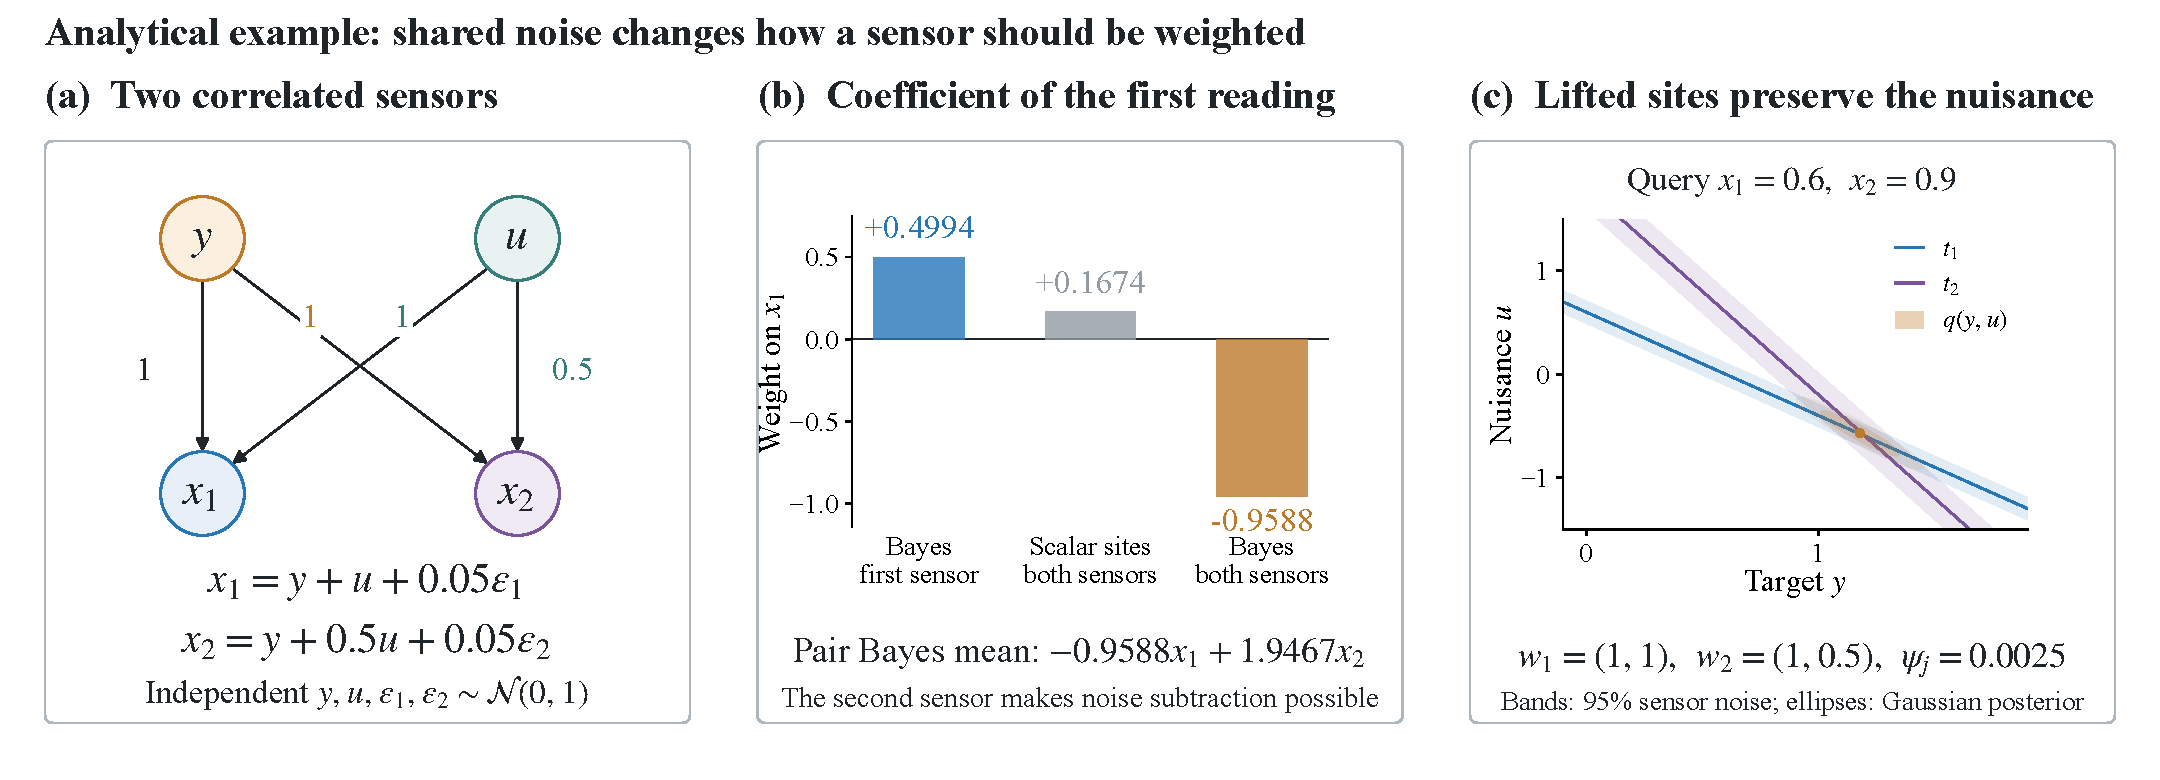
\includegraphics[width=\textwidth]{figures/shared_noise_example.pdf}
\caption{\label{fig:shared-noise}Analytical illustration of shared noise. Both sensors respond positively to the target, but they respond differently to the common disturbance. A single reading mixes these two sources. Their joint reading can separate them, allowing the first sensor's conditional coefficient to become negative. The coefficients are calculated from the stated Gaussian model and are not empirical performance measurements.}
\end{figure*}

This proposition applies to static Gaussian experts over the scalar target. A factor that receives the full observed subset, a factor whose parameters depend on a joint cavity, or an expert over a richer latent state has additional information and is not covered by this result. The motivation for lifting is therefore constructive: retain the convenient product representation while giving it a state in which the common disturbance can be represented explicitly.

\subsection{Exact fusion in a lifted state}

Let \(z=(y,h)\), where \(h\in\R^K\) represents shared nuisance variation. Assume
\begin{equation}
\begin{aligned}
 y&\sim\N(\mu_y,v_y),\qquad h\sim\N(0,I_K),\\
 x_j&=A_jy+D_j^\top h+c_j+e_j ,
\end{aligned}
\label{eq:lifted-generative}
\end{equation}
with \(y\) and \(h\) independent, \(v_y>0\), and mutually independent \(e_j\sim\N(0,\psi_j)\), \(\psi_j>0\), independent of \(z\). Write \(w_j=(A_j,D_j)\), \(o_j=x_j-c_j\), and the prior natural parameters as \((\Lambda_0,\eta_0)\). Sensor \(j\)'s likelihood contributes
\begin{equation}
 \Lambda_j=\frac{w_jw_j^\top}{\psi_j},
 \qquad \eta_j=\frac{w_jo_j}{\psi_j}.
 \label{eq:site}
\end{equation}
Its precision contribution has rank at most one and is positive semidefinite. The complete precision is positive definite because the prior is proper. The natural parameters combine by addition:
\begin{equation}
\begin{aligned}
 \Lambda_S&=\Lambda_0+\sum_{j\in S}\Lambda_j,\\
 \eta_S&=\eta_0+\sum_{j\in S}\eta_j,\\
 q(z\mid x_S)&=\N(\Lambda_S^{-1}\eta_S,\Lambda_S^{-1}).
\end{aligned}
\label{eq:product}
\end{equation}

\begin{proposition}[Exactness]
\label{prop:exact}
Under Eq.~\eqref{eq:lifted-generative}, the Gaussian in Eq.~\eqref{eq:product} is exactly \(p(z\mid x_S)\) for every fixed subset \(S\), including the empty subset. Its target marginal is the Bayes predictive distribution when the observation mask supplies no additional information about the target or nuisance state conditional on the observed readings.
\end{proposition}

The result follows by expanding the quadratic form of each Gaussian likelihood. Missing sensors have no observed likelihood, so they contribute no site. The nuisance is then integrated out by taking the target marginal of the joint Gaussian. This is ordinary exact Gaussian conditioning expressed in a form that exposes the sensor contributions. The architectural choice is to preserve that form when the contributions are learned.

The qualification about masks is statistical. If a sensor is more likely to fail at high target values, the event of failure can itself contain evidence. In that case the relevant posterior also includes a likelihood for the mask. Omitting an unobserved value remains a well defined computation, but it does not account for information carried by the selection mechanism. Likewise, fitting the anchor from a short support set gives a plug in model. Exact inference in that fitted model does not integrate uncertainty over its estimated parameters.

\subsection{When the nuisance dimension is necessary}

Sufficiency follows directly from the factor model: a shared disturbance of dimension \(K\) can be represented with \(K\) nuisance coordinates. A converse requires specifying the family of admissible sites. If site parameters can depend arbitrarily on all readings and the selected subset, they can encode information beyond a static factor model. The following result concerns fixed linear Gaussian measurement sites.

\begin{proposition}[Lifting dimension]
\label{prop:rank}
Let \(x=ay+Du+e\), where \(y\sim\N(0,1)\) and \(u\sim\N(0,I_K)\) are independent, and the Gaussian errors \(e_j\) are mutually independent, independent of \(y,u\), and have positive variance. Assume every \(a_j\ne0\). Write \(L=[a,D]\), and suppose that after deleting any row, \(L\) contains two disjoint nonsingular \((1+K)\) by \((1+K)\) submatrices.

Consider a proper Gaussian prior over \(z=(y,h)\), \(h\in\R^{K'}\), and static sites of the form in Eq.~\eqref{eq:site}, with \(o_j=x_j-c_j\), fixed \(w_j,c_j\), and positive fixed \(\psi_j\), all independent of readings and subsets. If their target marginal reproduces \(p(y\mid x_S)\) for every reading and every subset with \(|S|\le2\), then \(K'\ge K\).
\end{proposition}

For almost every loading matrix \(L\), the stated condition holds once \(P\ge2K+3\). The proof first reconstructs the sensor covariance from the empty, singleton and pair conditionals. It then uses the disjoint full rank submatrices to identify the diagonal uniquenesses of the factor decomposition, following the classical identifiability argument of Anderson and Rubin~\citep{anderson1956statistical}. A model with fewer latent coordinates cannot reproduce the resulting covariance. The full derivation is in Appendix~\ref{app:proofs}.

For the principal synthetic setting, \(K=1\) and \(P=5\). Under the generic condition, one shared nuisance coordinate is both sufficient and necessary within the static site family. This observation explains the choice of a small lifted state. It does not prescribe the latent dimension for arbitrary nonlinear sensor networks or replace model selection in a new application.

\subsection{Properties of the learned construction}

The compact cavity network described in Section~\ref{sec:method} changes the site parameters using calibration information and cavity moments. Its outputs still define positive semidefinite precision contributions, but its learned predictive distribution need not be the exact posterior of the original physical model. Several useful construction properties remain.

\begin{proposition}[Structural properties]
\label{prop:struct}
For every setting of the learned parameters, readings of missing query sensors do not affect the prediction. The same shared site network can be applied at any sensor count. Conditional on fully equivariant support statistics and consistently oriented anchor parameters, jointly permuting sensors and their calibration columns leaves the prediction unchanged. If the correction head is zero, every cavity round reproduces the Gaussian predictor of the fitted anchor.
\end{proposition}

The first property follows because sites of missing sensors are masked out of the aggregate and therefore out of the cavities used to update observed sensors. Computing a local feature for a masked slot does not make its reading part of the fused evidence. The second follows from sharing the per sensor maps and using sums of natural parameters. The permutation property also requires the anchor representation to transform consistently. A factor loading and its sign reversed counterpart describe the same Gaussian model, but a generic learned map can respond differently to the two coordinates. This distinction is relevant to the original implementation and its replay audit, which is discussed in Appendix~\ref{app:provenance}.

The final property gives training a meaningful starting point. A zero correction head represents the support fitted closed form exactly, so the model class contains that predictor. Consequently the infimum of training risk over the class cannot exceed the anchor's training risk. This is a statement about representation, not a guarantee about optimization or performance on a new deployment. The empirical comparisons test whether learning makes useful use of the available corrections.
